% !TEX root = ../report.tex
\chapter{Konzept}
\begin{Spacing}{\mylinespace}

\section{Modularisierung}
Um eine parallele Entwicklung und spätere Erweiterbarkeit sicherzustellen entschieden wir uns für eine modellbasierte Entwicklung.
Unser Projekt lässt sich in 3 Kategorien gliedern. Das ParticleSystem \textbf{(ParticleSystem)}, die Kinect Ansteuerung \textbf{(SandstormKinect)} und einen Controller \textbf{(Sandstorm)} der Events entgegen nimmt und diese verarbeitet oder ggf. weiterleitet.
Das XNA-Framework unterstützt einen modellbasierten Ansatz indem es jeder DrawableGameCompontent ihren eigenen Kontext zuweist.
Dies bedeutet das jede DrawableGameCompontent ein eigenes kleines Projekt darstellt und unabhängig von den anderen Projekten betrieben werden kann.
\begin{figure}[h!]
	\centering
	\vspace*{20px}
	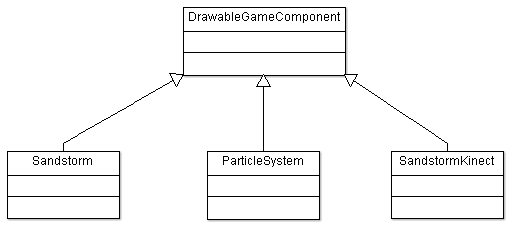
\includegraphics[width=320px]{graphics/DrawableGame.png}
	\caption{Kompontenten}
	\label{fig:singleColor}
\end{figure}


\end{Spacing}
\newpage
\clearpage
%% End Of Doc